\vspace{-.15in}\section{Research Plan and Methodology}
\label{sec:rep}\vspace{-.075in}

This \xxx project strenghens the reliability of datacenter computing with a 
holistic, thorough methodology. To this end, this section first proposes a 
fast, scalable consensus protocol (\S\ref{sec:protocol}). With this protocol, 
it presents a scheduler that makes general applications fault-tolerant 
(\S\ref{sec:scheduler}) and a new VM replication architecture (\S\ref{sec:vm}). 
The first two objectives include preliminary results. Finally, this section 
describes our research plan (\S\ref{sec:plan}).

\vspace{-.15in}\subsection{Objective 1: Building Fast, Scalable Consensus via
RDMA} 
\label{sec:model}\vspace{-.075in}

% P1: as mentioned in background, a key reason is thread interleavings, 
% so we need to reason about the general patterns we have. Or we say our 
% methodology is just like pattern matching.
Traditional \paxos protocols incur high consensus latency because they run on 
TCP/IP, which go through OS kernels and software network layers. In this 
section, \S\ref{sec:problem} analyzes this latency problem and its poor 
scalability in detail, and then presents our new RDMA-based \paxos 
protocol called \falcon (\S\ref{sec:falcon}).

\vspace{-.15in}\subsubsection{Problem: Consensus Latency of existing \paxos 
protocols scale poorly} 
\label{sec:examples}\vspace{-.075in}

% First, mainly introduce the problems in traditional protocols.
Due to the strong fault-tolerance of \paxos, it is widely served in many 
systems. For instance, Scatter~\cite{scatter:sosp11} runs 8$\sim$12 replicas in 
each \paxos group to order client requests, and it lets replicas respond 
requests in parallel. A bigger group size will improve Scatter throughput. 
Moreover, recent state machine replication (SMR) 
systems~\cite{eve:osdi12,rex:eurosys14,crane:sosp15} use \paxos to greatly 
improve the availability of
general server programs.

Unfortunately, despite these great advances, the high consensus latency of 
\paxos makes systems suffer. For efficiency, \paxos typically assigns one 
replica as the leader to invoke consensus requests, and the other replicas as 
backups to agree on requests. To agree on an input, at least one message 
round-trip is required between the leader and a backup. A round-trip causes big 
latency as it goes through TCP/IP layers such as software network stack and OS 
kernel. This latency could be acceptable for leader 
election~\cite{chubby:osdi,zookeeper} or
heavyweight transactions~\cite{crane:sosp15,eve:osdi12}, but undesirable for
key-value stores~\cite{redis,memcached}.

As replica group size increases, \paxos consensus latency often increases
drastically~\cite{scatter:sosp11} due to the linearly increasing number of 
consensus messages. One common approach to improve \paxos scalability is 
leveraging parallel techniques such as multithreading~\cite{zookeeper, 
spaxos:srds12} or asynchronous IO~\cite{crane:sosp15, libpaxos}. However, the 
high TCP/IP round-trip latency still exists, and synchronizations in these 
techniques frequently invoke expensive OS events such as context switches. We 
ran four \paxos-like protocols~\cite{zookeeper, spaxos:srds12, crane:sosp15, 
libpaxos} on 40Gbps network with only one client sending consensus requests. We 
found that, when replica group size increased from 3 to 9, the consensus 
latency of three protocols increased by \tradlatencyincreaselow to 
\tradlatencyincreasehigh, and \systemcostlow to \systemcosthigh of the increase 
was in OS kernel.

% Second, briefly mention the problem in DARE. and its scalability bottleneck.
As RDMA becomes increasingly popular and cheap, it becomes a promising approach 
to address the \paxos scalability problem. However, due to the unrich RDMA 
operation types, fully exploiting RDMA speed in software systems is widely 
considered challenging by the community~\cite{pilaf:usenix14,herd:sigcomm14,
farm:sosp15,dare:hpdc15}. For instance, \dare~\cite{dare:hpdc15} presents a
two-round, RDMA-based \paxos protocol in a sole-leader manner: leader does all 
RDMA workloads and backups do nothing. \dare was fast with 3 or 5 
replicas. However, our evaluation shows that, as replica group grows, the 
leader met scalability bottlenecks (\eg, polling ACKs). \dare's consensus 
latency increased by \darescalability as the group grows by 35x
(\S\ref{sec:eval-dare}).

\vspace{-.15in}\subsubsection{Falcon: a fast, scalable RDMA-based \paxos 
protocol} 
\label{sec:falcon}\vspace{-.075in}

Our key observation is that we should carefully separate RDMA workloads among
the leader and backups, especially in a scalability-sensitive context. 
Intuitively, we can let both leader and backups do RDMA writes directly on 
destination replicas' memory, and let all replicas poll their local memory to 
receive messages.

Although doing so will consume more CPU resources than a sole-leader 
protocol~\cite{dare:hpdc15}, it has three major benefits. First, the leader 
has less workloads. Second, both leader and backups participate in consensus, 
which makes it possible to reach consensus with only one 
round~\cite{paxos:practical}. Third, all replicas can get rid of 
the expensive RDMA ACK polling and just receive consensus messages on their 
bare, local memory. An analogy is threads receiving other threads' data via 
bare memory, a fast and scalable computation pattern.

We present \xxx,\footnote{We name our system after
falcon, one of the fastest birds.} a new RDMA-based \paxos protocol and its
runtime system. In \xxx, all replicas directly write to destination
replicas' memory and poll messages from local memory to receive messages, and 
our runtime system handles other technical challenges such as message 
atomicity (\S\ref{sec:normal}), efficient input logging (\S\ref{sec:logging}), 
and failure recovery (\S\ref{sec:checkpoint}).

Inheritated from our general SMR system \crane~\cite{crane:sosp15}, \xxx's 
design supports general, unmodified server programs. Within \xxx, a program 
runs as is. \xxx automatically deploys this program on replicas, intercepts 
inputs from a server program's inbound socket calls (\eg, \recv) with a Linux 
technique called LD\_PRELOAD, and invokes its \paxos protocol to enforce same 
inputs across replicas.

% Three figures. First, falcon arch. Second, consensus protocol. Third, falcon 
% results compared to traditional ones and DARE.

\begin{figure}[!htb]
    \begin{minipage}{.49\textwidth}
        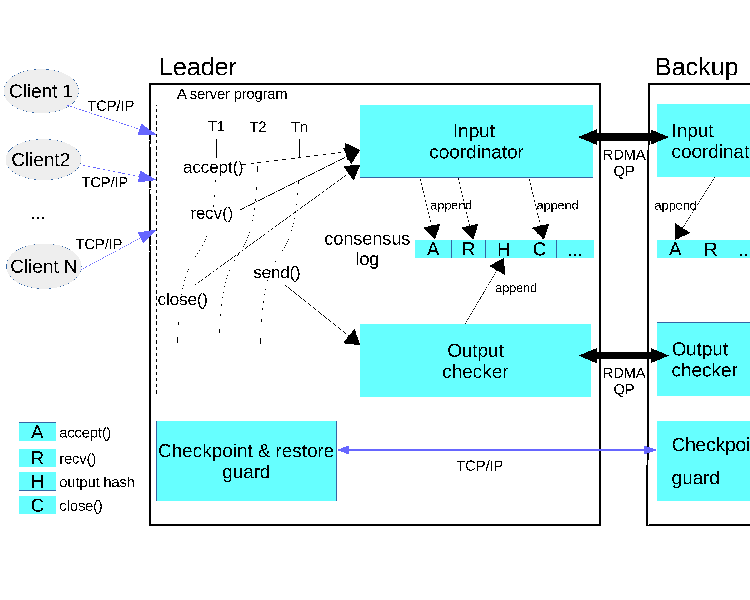
\includegraphics[width=0.34\textheight]{figures/arch.ps}
        \vspace{0.1in}
        \caption{The \falcon architecture.}
        \label{fig:falcon-arch}
    \end{minipage}
    \begin{minipage}{0.51\textwidth}
        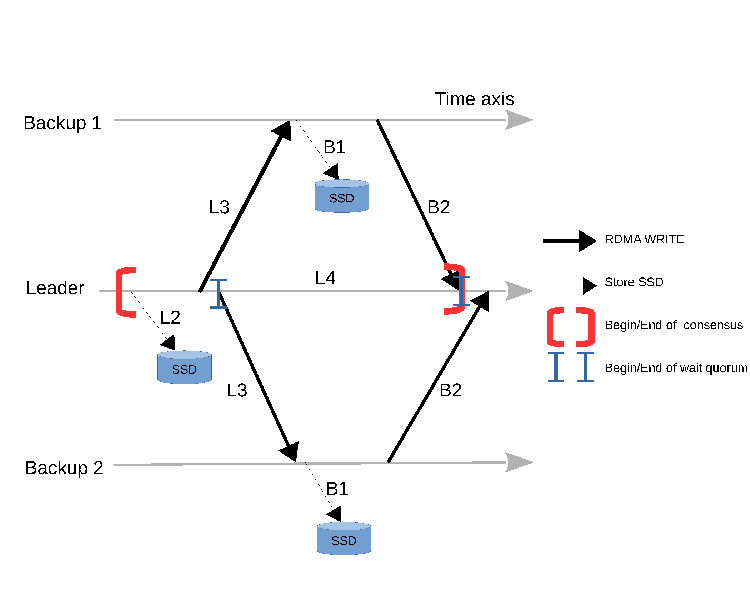
\includegraphics[width=0.34\textheight]{figures/consensus.ps}
        \vspace{0.1in}
        \caption{\falcon protocol in normal case.}
        \label{fig:falcon-protocol}
    \end{minipage}
\end{figure}

\para{Primilinary results.} Crane. Falcon. Say Crane is first version. Falcon 
totally subsumes Crane. Falcon also has initial results.

\begin{figure}[!htb]
\centering
\includegraphics[width=0.34\textheight]{figures/traditional_paxos_latency.ps}
        \vspace{0.1in}
        \caption{Consensus latency of six \paxos protocols. \falcon is fastest 
and scales the best.}
        \label{fig:scalability}
\end{figure}

\para{Future work.} Evaluate its scalability on thousands or even more 
machines. Evaluate its generality on more applications. Evaluate the RDMA-based 
failure recovery sub-protocols on various failure scenarios.

\vspace{-.15in}\subsection{Objective 2: 
Integrating Falcon with Datacenter Schedulers}\label{sec:detect}\vspace{-.075in}

A naive approach to achieve high-availability for critical applications could 
be integrating \paxos within every application. However, this integration 
approach has two major issues. First, \paxos is notoriously difficult 
to understand~\cite{raft:usenix14}, implement~\cite{paxos:practical}, and 
verify~\cite{demeter:sosp11}.

Second, running a \paxos-enabled application with a 
cluster management system can be problematic because the system is unaware 
of replication logic. For instance, if an application submits three copies of 
the same job to the system, the system may happen to schedule all three 
copies on the same machine (although it should schedule them on 
different machines to tolerate machine failures).

\vspace{-.15in}\subsubsection{\tripod: the fault-tolerant scheduler 
architecture} 
\label{sec:scheduler-arch}\vspace{-.075in}

This paper proposes the design of \tripod,\footnote{We name our system after 
the ancient Chinese three-legged tripod, a reliable, multi-purpose container.} 
a cluster management system that automatically provides high-availability to 
general applications. \tripod maintains replicas of controllers with a new 
RDMA-enabled \paxos protocol~\cite{falcon:github}. Unlike existing systems 
which let only the leader controller schedule jobs, \tripod runs replicas of 
the same job using the replicas of controllers: after controllers agree on a 
new job, \tripod lets each controller schedule an independent copy of this job.

To avoid the two aforementioned integration issues, \tripod chooses to 
integrate 
\paxos in the cluster system, not in applications. Doing so has two benefits. 
First, \tripod's \paxos acts as a single, general SMR service to applications. 
We 
can just leverage existing verification 
tools~\cite{modist:nsdi09,demeter:sosp11} to make sure that this \paxos 
protocol is robust and correct, and then we can benefit many applications. 
Second, now \tripod's own scheduler can handle the replication logic and do 
careful, replication-aware scheduling for jobs.

In an implementation level, \tripod integrates \mesos~\cite{mesos:nsdi11}, a 
widely 
used cluster management system, with a new RDMA-enabled \paxos 
protocol~\cite{falcon:github}. Compared to a prior RDMA-enabled \paxos 
protocol~\cite{dare:hpdc15}, our new protocol can support general programs 
transparently without modifications.

Figure~\ref{fig:arch} depicts \tripod's architecture, and its key components 
are 
shaded (and in blue). To illustrate how \tripod works in an application 
perspective, this figure shows two applications, Hadoop and MPI. Each 
application has a \emph{replica strength} (\v{R}) to denote the level of 
fault-tolerance it demands. This value is either 1 or equals the number of 
replicas of controllers in \tripod.

By default, each application has \v{\v{R}=1}, which means that this application 
does not need replication. For such a default setting, \tripod runs the job as 
is 
without replication, like a typical cluster management system (\eg, Mesos).

In this figure, Hadoop's \v{R} is 3, which means that it wants to replicate 
each of its job with three copies for high-availability. Suppose Hadoop 
submits two jobs to the leader controller, each has different shapes (triangle 
or hexagon). The leader controller then invokes a consensus on each job across 
controllers. Once a consensus is reached, each controller assigns the same job 
on different slave machines.

The leader controller directly returns its computation result to the Hadoop 
scheduler unless a tail-tolerance mechanism is triggered 
(\S\ref{sec:workflow}). 
Standby controllers ignore the results unless the same mechanism is triggered.

\vspace{-.15in}\subsubsection{The replication-aware resource allocation scheme}
\label{sec:detect-arch}\vspace{-.075in}

Figure~\ref{fig:workflow} shows \xxx's workflow on scheduling jobs with four 
steps. This workflow is similar to that in Mesos except the second and fourth 
steps. These two steps \tripod abstract away the replication logic in its 
resource offers and allocations from the application. An application runs as if 
\xxx does not replicate any of its jobs, and \tripod transparently handles all 
the replication logic.

In the first step, slave machines periodically report their available computing 
resources (\eg, CPU cores and memory) to the leader controller. In the second 
step, instead of offering the available resources aggregated from slave 
machines, \tripod divides the amount of resources by each application's \v{R} 
value and then sends a resource offer to the application. The goal is to 
reserve enough resources for \tripod to replicate a job with \v{R} copies.

In the third step, an application scheduler submits jobs to the leader 
controller. The leader controller then invokes a consensus on this job by 
carrying the resource offer made to the application.

Once a majority of controllers agrees on executing this job, each controller 
does the fourth step. It schedules this job on an available slave machine 
according to the resource offer. To prevent controllers putting the same job on 
the same slave machine, the leader controller first makes an assignment on 
which controller should run this job on which slave machine, it then carries 
this assignment in its consensus request. Once a consensus on this job is 
reached, each controller follows this assignment.

Two figures: one is TRIPOD arch. The other is TRIPOD results from the workshop 
paper. Figure~\ref{fig:scheduler-arch} and Figure~\ref{fig:scheduler-workflow} 
and Figure~\ref{fig:scheduler-latency}.


\para{Reliability v.s. resource consumption} The main goal of \xxx is to 
provide high-availability to critical applications 
running in clusters. On one hand, clusters are included more and more computing 
resources (\eg, machines), where failures of these resources and applications 
are already commonplace~\cite{facebook:outage}. On the other hand, 
high requirements on response times and availability become more and more 
important to critical applications.

For instance, Both NYSE and Nasdaq have experienced outage of their whole 
site~\cite{nyse:halt} or specific IPO events~\cite{facebook:ipo:delay} due to 
minor machine errors.  Even social-networking applications like Facebook has 
strong fault-tolerance requirements, because minor machine failures have turned 
down the whole Facebook site for several times in the last few 
years~\cite{facebook:outage}, costing huge 
money lost. 

Therefore, \tripod's design favors more on availability and performance 
(low consensus latency). It's design tends to use \v{R} times of resources 
compared to traditional applications. We argue that this extra resource 
utilizations are acceptable for critical applications, because if they have 
high 
demand on availability and response times, they can often tolerate costs on 
computing resources (\eg, trading and medical platforms).

\begin{figure}[!htb]
    \begin{minipage}{.49\textwidth}
        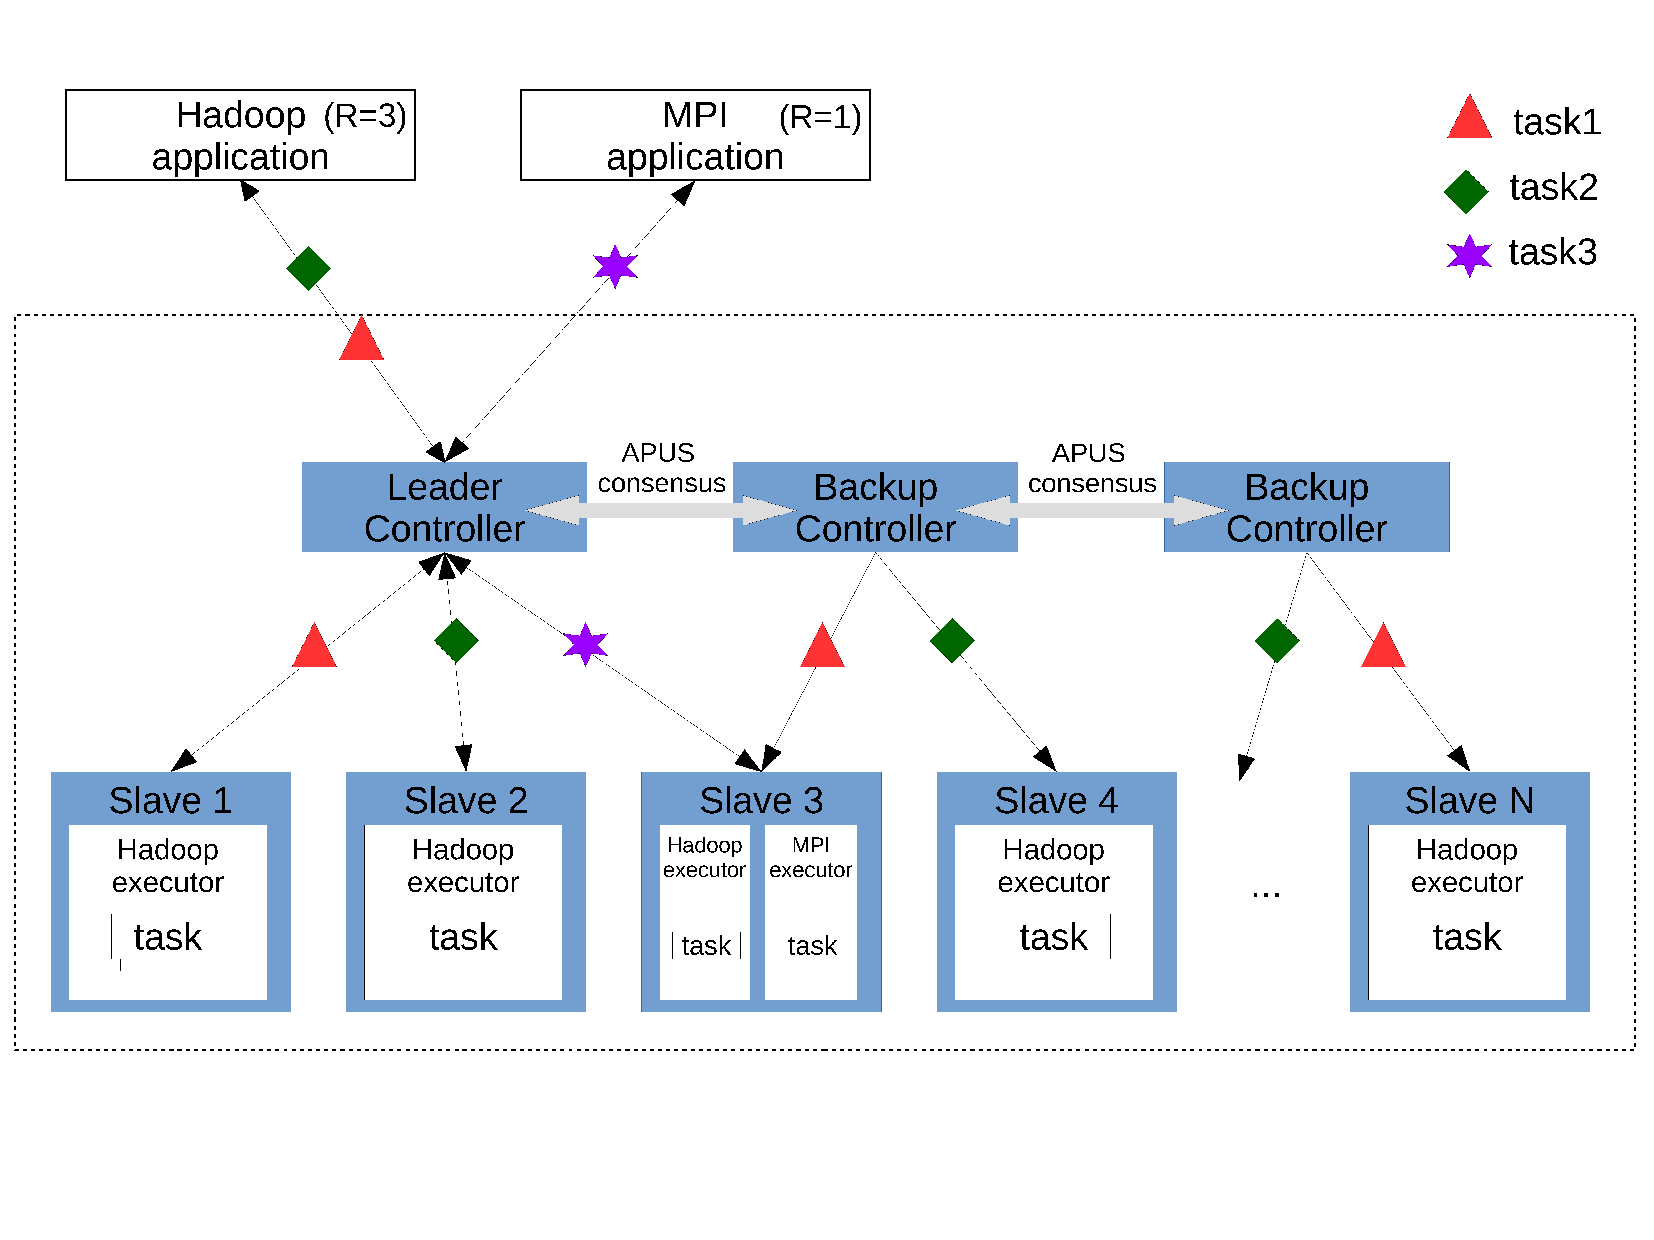
\includegraphics[width=0.34\textheight]{figures/scheduler_arch.ps}
        \vspace{0.1in}
        \caption{Fault-tolerant scheduler.}
        \label{fig:scheduler-arch}
    \end{minipage}
    \begin{minipage}{0.51\textwidth}
        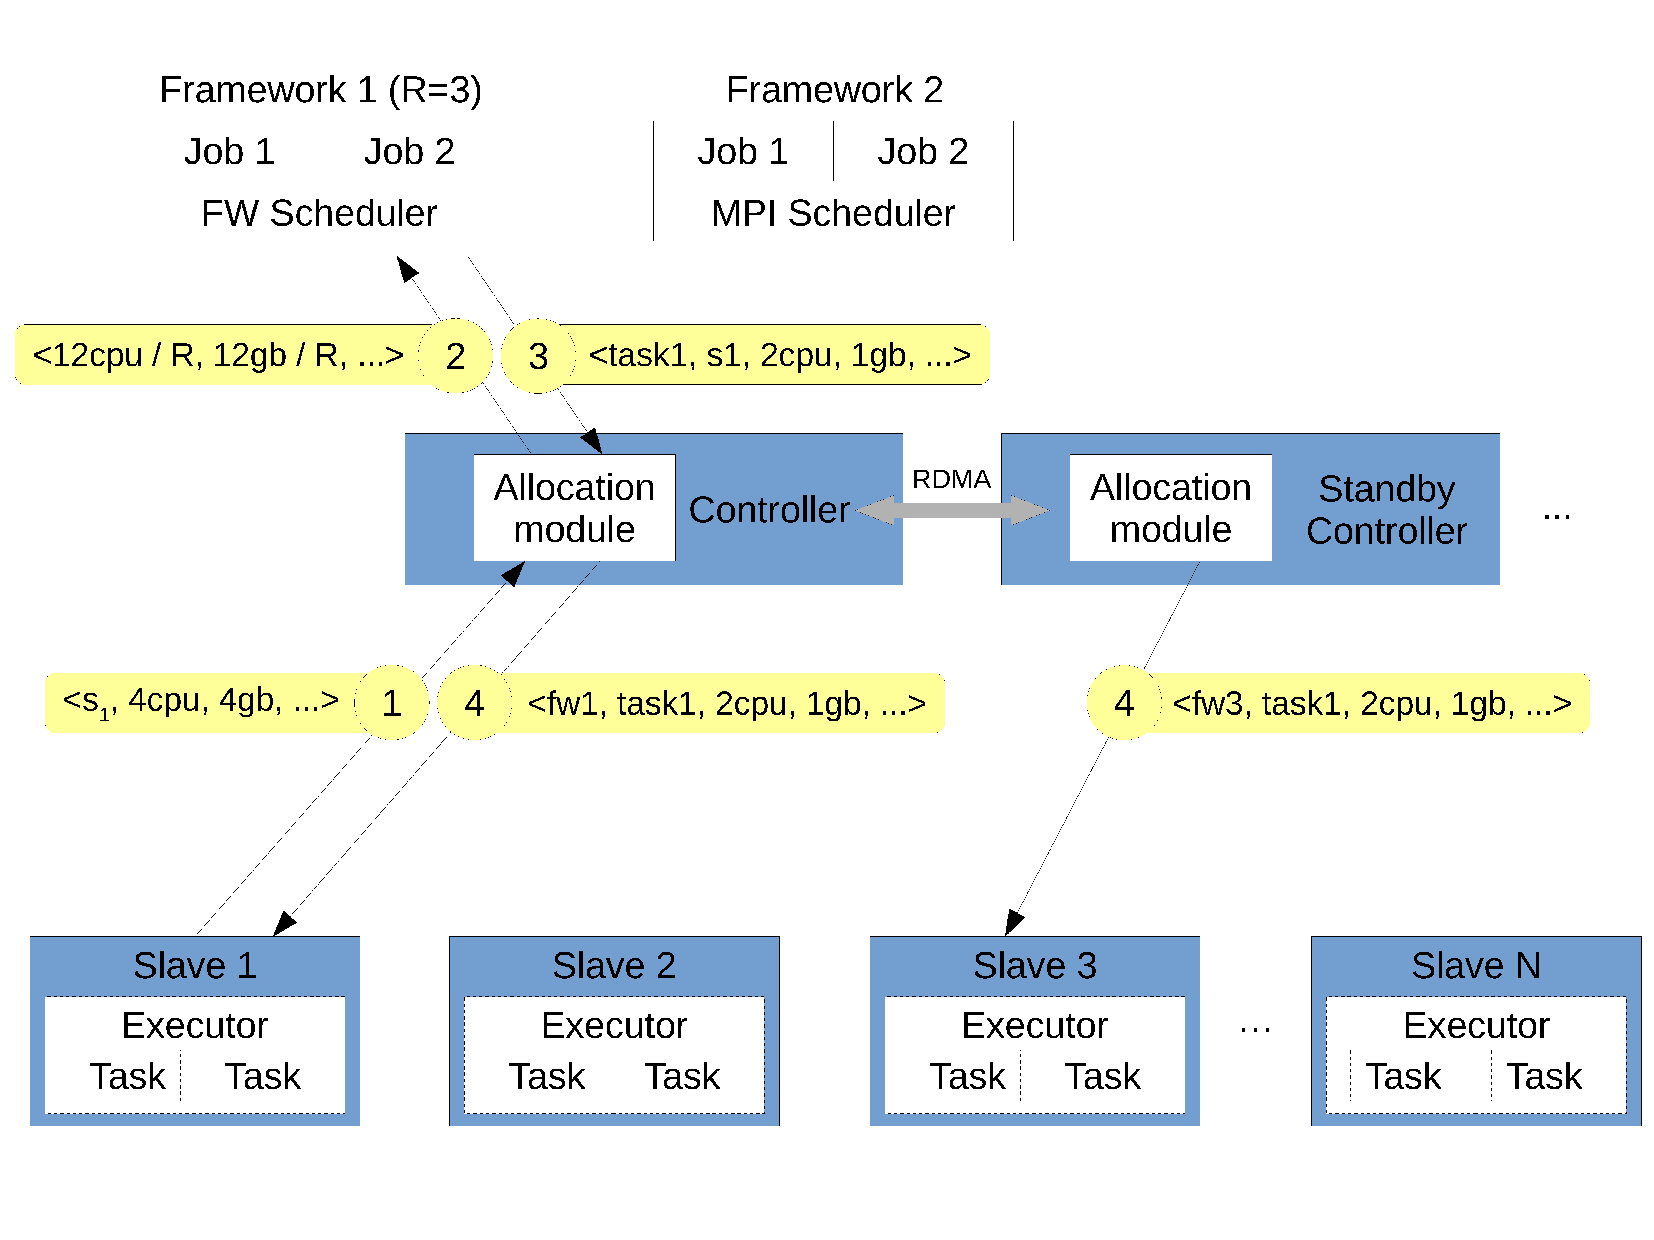
\includegraphics[width=0.34\textheight]{figures/scheduler_flow.ps}
        \vspace{0.1in}
        \caption{Workflow.}
        \label{fig:scheduler-workflow}
    \end{minipage}
\end{figure}

\para{Primilinary results.} change redis to memcached. used in financial 
platform and social networking.

To emulate a typical social-networking application, we ran this protocol with 
\redis~\cite{redis}, a popular key-value store used by Twitter. Evaluation 
showed that, compared to \redis's unreplicated execution, \xxx incurred merely 
a \tputoverhead overhead in throughput and \latencyoverhead in response time. 
This protocol was 40.1X faster than a \zookeeper-based
SMR protocol~\cite{calvin:sigmod12} which runs on TCP/IP.

\begin{figure}[!htb]
\centering
\includegraphics[width=0.34\textheight]{figures/scheduler_latency.ps}
        \vspace{0.1in}
        \caption{Performance overhead of scheduler.}
        \label{fig:scheduler-latency}
\end{figure}

\para{Open challenges.} New algorithm on scheduling and replication. Others? 
Apply them to do tail tolerance.

\vspace{-.15in}\subsection{Objective 3: 
Strenghening VM to improve application 
availability}\label{sec:defense}\vspace{-.075in}


% TBD: need a new replication approach name.
\vspace{-.15in}\subsubsection{Idea I: Hybrid Replication} 
\label{sec:defense-arch}\vspace{-.075in}

TBD.

\vspace{-.15in}\subsubsection{Idea II: \paxos-based Live Migration} 
\label{sec:defense-arch}\vspace{-.075in}

TBD.

\vspace{-.15in}\subsection{Research Plan} \label{sec:plan}\vspace{-.075in}

This project will require two PhD students S1 and S2 to work for 
three years. In the first year, S1 will develop and refine the concurrency 
attack model (part of \textbf{Objective~1}), and S2 will leverage the model to 
design the detailed workflow of the detection approach (part of 
\textbf{Objective~2}) by working closely with S1. In the second year, S1 will 
do an empirical study on how well the model represents real-world concurrency 
attacks (part of \textbf{Objective~1}), and S2 will implement the detection 
approach as a software tool (part of \textbf{Objective~2}). In the third year, 
S1 will implement the defense infrastructure (\textbf{Objective~3}), and S2 
will study the detection tool on a broad range of real-world multithreaded 
programs to find new attacks.
% Both students will 
% involve theoretical methods, implement real software systems, and 
% perform real-world study.
% The PI will supervise the students by providing 
% advice concerning both theoretical and systems implementation levels.


